\documentclass{article}
\usepackage[english, magyar]{babel}
\usepackage{t1enc}
\usepackage[inline]{enumitem}
\usepackage{hulipsum}
\usepackage{graphicx}
\usepackage{xcolor}

\begin{document}
	\begin{titlepage}
		\title{\Huge{\textit{Bevezetés a \LaTeX -be}}}
		\author{\Large{Harmadik alkalom}}
		\maketitle
	\end{titlepage}

\tableofcontents
\clearpage

\section{feladat - "Egysoros lista"}
\begin{enumerate}
	\item [!]First item with enumerate
	\item [?]Second item with enumerate
	\item [és]third item with enumerate
\end{enumerate}

\section{feladat - Számozott lista}
\begin{enumerate}
	\item Első szint
	\begin{enumerate}
		\item Második szint
		\begin{enumerate}
			\item [-]Harmadik szint
			\begin{enumerate}
				\item [-]Negyedik (utolsó) szint
			\end{enumerate}
		\end{enumerate}
	\end{enumerate}
\end{enumerate}

\hulipsum[2]

\begin{enumerate}[label=\textbullet]
	\item Első számozás
	\item [-]Második számozás
	\item Harmadik számozás
\end{enumerate}
\clearpage

\section{feladat - Leíró lista}
\begin{description}[align=parleft,%
	leftmargin=*,widest={hosszabb}]
	\item[slanted]
	\item[rövid cimke] \hulipsum[2]
	\item[hosszú cimke!] \hulipsum[3]
\end{description}
\clearpage

\section{feladat - Ábrák}

\hulipsum[1]

\begin{figure}[bt] %figurben lévőket nem lehet megtörni
	\centering
	\label{fig:kepek}
	\caption{Felirat/képaláírás}
	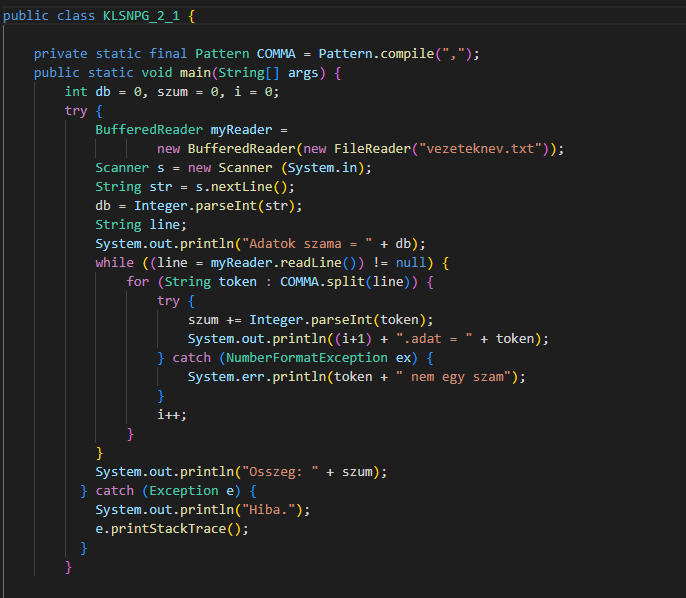
\includegraphics[width=0.5\linewidth]{1}
	\caption{Felirat/képaláírás}
	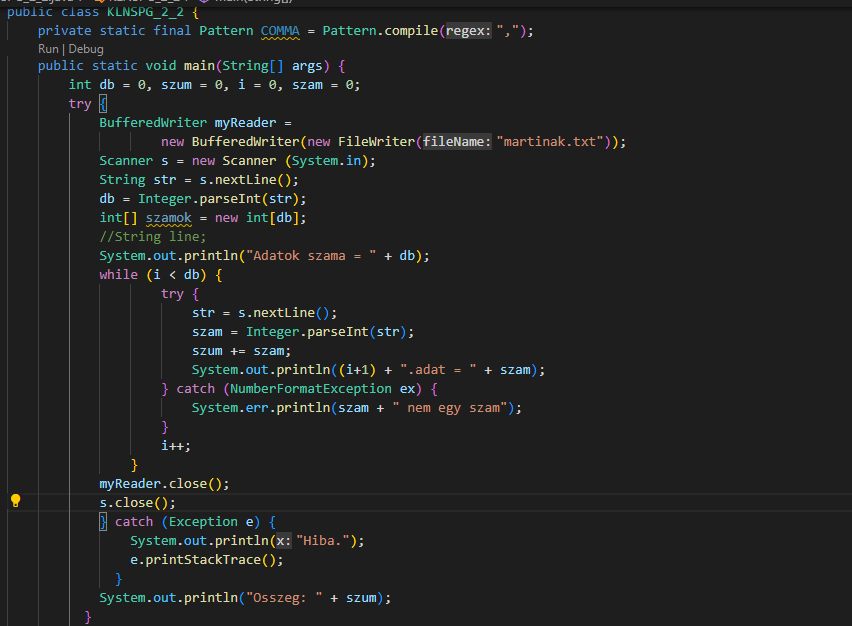
\includegraphics[width=0.5\linewidth, angle = 90]{2}
\end{figure}

\hulipsum[1]

\section{feladat - Táblázatok}
\begin{tabular}{|p{3cm} | p{5cm} |}
	\hline
	Hello& \LaTeX
\end{tabular}


\end{document}